


%% Goal is 

\section{Introduction}
\label{sec:GUI:introduction}
There are many reasons why one would want to create a graphical user
interface for a package or piece of \R\/ functionality. For example,
% ML: I think many of these points are debateable, at best. The CLI is
% extremely flexible and provides the easiest general access to
% R. GUI's are best constrained to focused tasks and are particularly
% well-suited for casual users who are not familiar with the R
% language and the command line interface. The one about integration
% with graphics (presumably to create interactive visualizations) is a good one.

%% JV: agreed. Let's try these:
\begin{itemize}
%\item GUIs allow others easier access to your functions,
%\item GUIs are useful if a function has many arguments,
\item GUIs can make \R's functionality available to the casual \R\/ user,
\item GUIs can be dynamic, they can direct the user how to fill in
  arguments, can give feedback on the choice of an argument, they can
  prevent or allow user input as appropriate,
\item Although a command line is usually faster when the commands are
  known, a GUI can make some less commonly used tasks easier to do.
\item GUIs make dealing with large data sets easier both visually and
  as an alternative to sometimes difficulte command line usage.
\item GUIs can tightly integrate with graphics, for example the
  rggobi interface among others.
\end{itemize}
% ML: It is not clear why we are arguing for a common, general GUI. The focus
% on the book seems to be the development of special-purpose GUI's.

% JV: I'm not (I hope). I just want to avoid it seeming like a waste of time
% to learn writing GUIs in case someone (say revolutions) writes such a
% general GUI. 
Even as \R\/ is rapidly gaining interest, especially commercial
interest, it lacks a common graphical user interface. This is due to
several reasons. (1) The \R\/ language is designed for command line
usage. (2) The GUI would need to run on all supported \R\/ platforms
(3) the wide variety of user types means a single interface would be
unlikely to satisfy all. Even if it did have a common interface, as
much of \R's functionality depends on user contributions there will
always be a demand for package programmers to provide convenient
interfaces to their work.



\XXX{Space}
\XXX{HCI}
\XXX{http://www.useit.com/alertbox}
\XXX{Apple HIG}
\XXX{comment on radio vs. check http://www.useit.com/alertbox/20040927.html}
\section{A simple GUI in R}
\label{sec:GUI:tic-tac-toe}
%% Tic Tac Toe examples

We begin with an example showing how one can use \R's standard
graphics device, as a canvas for drawing a GUI, for playing a game of
tic-tac-toe against the computer. Although this example
has nothing to do with statistics, it illustrates, in a familiar way,
some of the issues that this text will address with using GUIs. 


%% ML: the note about the MVC pattern can probably come after the
%% concrete model, view and controller have been presented. We can
%% look back and point out that the design of the example can be
%% generalized to MVC and that we will encounter such designs
%% throughout the book, even if it is not always explicit. It's OK to
%% generalize a little after each step, but I think we want to lead
%% with the concrete.

Many GUIs can be thought of as different views of some data
model. 
In this example, the data simply consists of information holding the
state of the game. Here we define a global variable, \code{board}, to store the
current state of the game. 

%% Model
\begin{Schunk}
\begin{Sinput}
 board <- matrix(rep(0,9), nrow=3)       # a global
\end{Sinput}
\end{Schunk}

%% View
The GUI provides the representation of the data for the user. This
example just uses a canvas for this, but most GUIs have a combination
of components to represent the data and allow for user
interaction. The layout of the GUI directs the user as to how to
interact with it and is an important factor as to whether the GUI will
be well received. Here we define a function to layout the game board
using the graphics device as a canvas.

\begin{Schunk}
\begin{Sinput}
 layoutBoard <- function() {
   plot.new()
   plot.window(xlim=c(1,4), ylim=c(1,4))
   abline(v=2:3);  abline(h=2:3)
   mtext("Tic Tac Toe. Click a square:")
 }
\end{Sinput}
\end{Schunk}

%% Controller
A GUI is designed to respond to user input typically by the mouse or
keyboard. The underlying toolkit allows the programmer to assign
functions to be called when some specific event occurs. Typically, the
toolkit \textit{signals} that some action has occurred, and then
calls \textit{callbacks} or \textit{event handlers} that have been
assigned by the programmer. How this is implemented varies from
toolkit to toolkit.

\R's interactive graphics devices implement the \code{locator}
function which responds to mouse clicks by user. When using this function,
one specifies how many mouse clicks to gather and the \textit{control}
of the program is suspended until these are gathered (or the process
is terminated). The suspension of control makes this a \textit{modal}
GUI. This design is common for simple dialogs that require immediate
user attention, but not common otherwise. To make non-modal dialogs
possible, the writers of the \R\/ packages that interface with the GUI
toolkits have to interface with \R's event loop mechanism.


Here we define a function to collect the player's input.
\begin{Schunk}
\begin{Sinput}
 doPlay <- function() {
   iloc <- locator(n=1, type="n")
   clickHandler(iloc)
 }
\end{Sinput}
\end{Schunk}

In the above function,
\function{clickHandler} is an \textit{event handler}. Its job is to process the output of the
\function{locator} function, checking first if the user terminated
\function{locator} using the keyboard. If not it proceeds to draw the
move, and then, if necessary, the computer's move. Afterwards, play is
repeated until there is a winner or a ``cat's'' game. 


\begin{Schunk}
\begin{Sinput}
 clickHandler <- function(iloc) {
   if(is.null(iloc)) 
     stop("Game terminated early")
   move <- floor(unlist(iloc))
   drawMove(move,"x")
   board[3*(move[2]-1) + move[1]] <<- 1
   if(!isFinished()) 
     doComputerMove()
   if(!isFinished()) 
     doPlay()
 }
\end{Sinput}
\end{Schunk}
%%>>

The use of \verb+<<-+ in the handler illustrates a typical issue in
GUI design within \R. After a GUI is created, the state is
typically modified within the scope of the callback functions. These
callbacks need to be able to modify values outside of their scope, yet
even if the values are passed in as argument, this is usually not
possible while assigning within the scope of the function call, due to
\R's pass by copy function calls. As such, global variables are often
employed along with some strategies to avoid an explosion of variable
names.

%% validation of user input
Validation of user input is an important task for a GUI, especially
for Web GUIS. In the above,
the \function{clickHandler} function checks to see if the user
terminated the game early and issues a message, more helpful forms of
validation are possible in general.

%% Implement logic
At this point, we have a data model, a view of the model and the
logic that connects the two, but we still need to implement some of the
functions to tie it together.


This function draws either an ``x'' or an ``o''. It does so using the
\function{lines} function. The \code{z} argument contains the
coordinates of the square to draw.
\begin{Schunk}
\begin{Sinput}
 drawMove <- function(z,type="x") {
   i <- max(1,min(3,z[1])); j <- max(1,min(3,z[2]))
   if(type == "x") {
     lines(i + c(.1,.9),j + c(.1,.9))
     lines(i + c(.1,.9),j + c(.9,.1))
   } else {
     theta <- seq(0,2*pi,length=100)
     lines(i + 1/2 + .4*cos(theta), j + 1/2 + .4*sin(theta))
   }
 }
\end{Sinput}
\end{Schunk}

%% Resizing
One could use \code{text} to place a text ``x'' or ``o'', but this may
not look good if the GUI is resized. Most GUI layouts allow for
dynamic resizing. Overall this is a great advantage, for example, it
allows translations to just worry about the text and not the layout,
which will be different for every language.

This function is used to test if a game is finished. The matrix
\code{m} allows us to easily check all the possible ways to get three
in a row.
\begin{Schunk}
\begin{Sinput}
 isFinished <- function() {
   if(sum(abs(board)) >= 9) 
     return(TRUE)
   m <- matrix(1:9,nrow=3)
   ways <- list(m[,1], m[,2], m[,3],
                m[1,], m[2,], m[3,],
                diag(m),diag(apply(m,2,rev)))
   sums <- sapply(ways, function(i) abs(sum(board[i])))
   if(any(sums == 3)) 
     return(TRUE)
   return(FALSE)
 }
\end{Sinput}
\end{Schunk}

This function picks a move for the computer.  The move is converted
into coordinates using \code{\%\%} to get the remainder and
\code{\%/\%} to get the quotient when dividing an integer by an
integer. This function just chooses at random from the left over
positions; we leave implementing a better strategy to the interested
reader.

\begin{Schunk}
\begin{Sinput}
 doComputerMove <- function() {
   newMove <- sample(which(board == 0),1) # random !
   board[newMove] <<- -1    
   z <- c((newMove-1) %% 3, (newMove-1) %/% 3) + 1
   drawMove(z,"o")
 }
\end{Sinput}
\end{Schunk}
%%>>


%% main equivalent
This function provides the main entry point for our GUI. To play a
game it first lays out the board and then calls
\function{doPlay}. When this function terminates, a message is written
on the screen.
\begin{Schunk}
\begin{Sinput}
 playGame <- function() {
   layoutBoard()
   doPlay()
   mtext("All done\n",1)
 }
\end{Sinput}
\end{Schunk}

This example adheres to the model-view-controller design pattern that
is implemented by virtually every complex GUI. We will encounter this
pattern throughout this book, although it is not always explicit.

%% endless tweak
A final point, the above example illustrates a common issue when designing
software that is particularly true of GUIs -- feature creep is an
endless temptation. In this case, there are many obvious improvements:
localizing the text messages so different languages can be used,
implementing a better logic for the computer's moves, drawing a line
connecting three in a row when there is a win, indicating who won when
there is a win, etc. For many GUIs there is a necessary trade-off
between usability and complexity.

\section{GUI Design Principles}
\label{sec:GUI:design}
% Section to introduce GUI design and principles through a comparison of
% three dialogs and general discussion


%% mac defs:

% Document windows contain file-based user data. They present a view
% into the content that people create and store. If the document is
% larger than the window, the window shows a portion of the document’s
% contents and provides users with the ability to scroll to other areas.

% Application windows are the main windows of applications that are not
% document-based. These windows can use the standard Aqua window look
% and features or (less frequently) the brushed metal look.

% Utility windows float above other windows and provide tools or
% controls that users can work with while documents are open. Utility
% windows (also called palettes) are discussed in more detail
% in “Utility Windows.” (page 202)

% Dialogs and alerts require a response from the user. These are
% discussed in “Dialogs.” (page 207)


The most prevalent pattern of user interface design is denoted WIMP,
which stands for Window, Icon, Menu and Pointer (i.e., mouse). The
WIMP approach was developed at Xerox PARC in the 1970's and later
popularized by the Apple Macintosh in 1984. This is particularly
evident in the separation of the window from the menubar on the Mac
desktop. Other graphical operating systems, such as Microsoft Windows,
later adapted the WIMP paradigm, and libraries of reusable GUI
components emerged to support development of applications in such
environments. Thus, GUI development in R adheres to WIMP approach.

The primary WIMP component from our perspective is the window. A
typical interface design consists of a top-level window referred to as
the \dfnref{document window} that shows the current state of a
``document'', whatever that is taken to be. In \R\/ it could be a data
frame, a command line, a function editor, a graphic or an arbitrarily
complex form containing an assortment of such elements. 

%% JV: control or "action" here?
%% ML: tried to make this clearer

Abstractly, WIMP is a command language, where the user executes
commands, often called actions, on a document by interacting with
graphical controls. Every control in a window belongs to some abstract
menu. Two common ways of organizing controls into menus are the
menubar and toolbar.

The parameters of an action call, if any, are controlled in
sub-windows. These sub-windows are termed \dfnref{application windows}
by Apple~\citep{APPLE:HIG}, but we prefer the term \dfnref{dialogs},
or \dfnref{dialog boxes}. These terms may also refer to smaller
sub-windows that are used for alerts or confirmation. The program
often needs to wait for user input before continuing with an action,
in which case the window is modal. We refer to these as \dfnref{modal
  dialog boxes}.

Each window or dialog typically consists of numerous controls laid out
in some manner to facilitate the user interaction. Each window and
control is a type of \textit{widget}, the basic element of a
GUI. Every GUI is constituted by its widgets. Not all widgets are
directly visible by the user; for example, many GUI frameworks employ
invisible widgets to lay out the other widgets in a window.

There is a wide variety of available widget types, and widgets may be
combined in an infinite number of ways. Thus, there are often numerous
means to achieve the same goals. For example,
Figures~\ref{fig:GUI:print-dialogs} and \ref{fig:GUI:print-dialogs-R} show three dialogs that perform
the same task -- collect arguments from the user to customize the
printing of a document. Although all were designed to do the same
thing, there are many differences in implementation.

%% ML: Print dialogs might be problematic, especially with Firefox, which
%% (through GTK+) will use the platform native print dialog. On Linux,
%% there is no native dialog, so GTK+ implements one. This might not
%% be true of Firefox 2.0 specifically, but that is getting old
%% now. What about taking the print dialog from the R Windows GUI?

%% Principles of GUI layout
%% http://www.sylvantech.com/~talin/projects/ui_design.html has a nice list

\begin{figure}
  \centering
  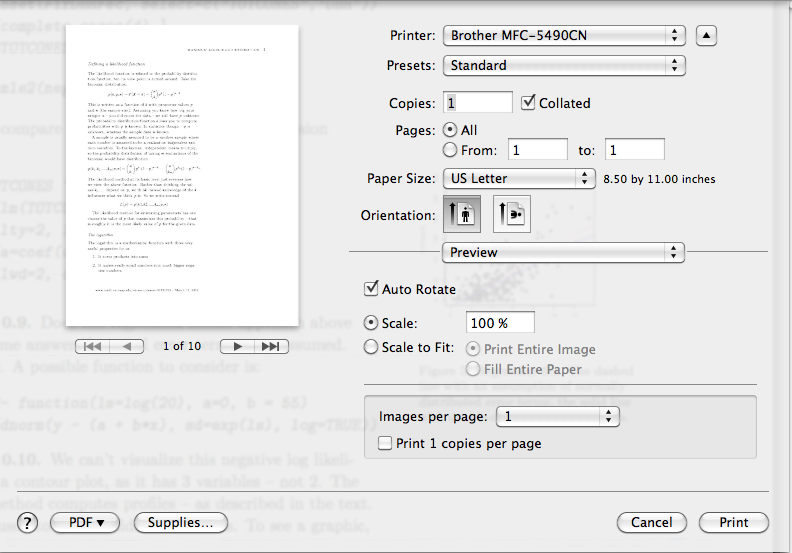
\includegraphics[width=.80\textwidth]{fig-mac-print}
   \\
   
  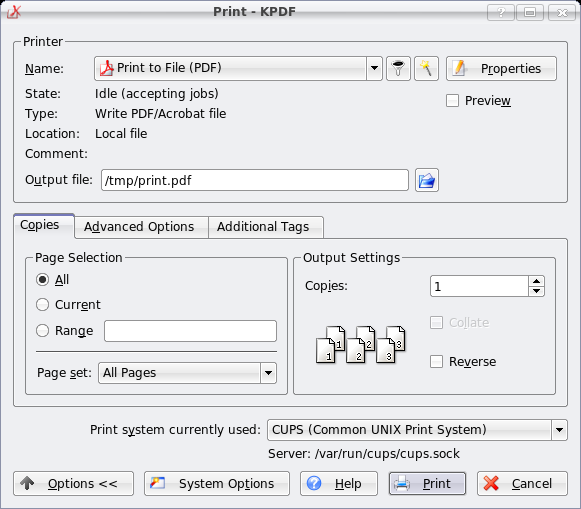
\includegraphics[width=.80\textwidth]{kde-print}
  \caption{Two print dialogs. One from Mac OS X 10.6 and one from KDE 3.5.}
  \label{fig:GUI:print-dialogs}
\end{figure}


\begin{figure}
  \centering
  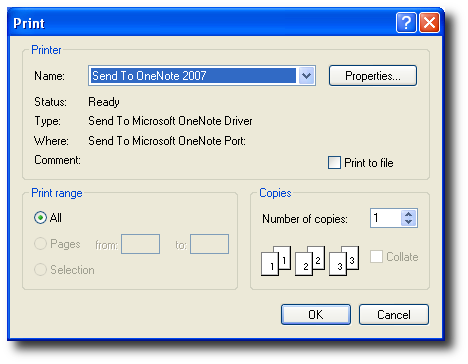
\includegraphics[width=.80\textwidth]{r-print-dialog}
  \caption{\R's print dialog under windows XP using XP's native dialog.}
  \label{fig:GUI:print-dialogs-R}
\end{figure}

%% Choice of widget -- familiar metaphors, use of icons, 
In some cases, typical usage suggests one control over another. The
choice of printer for each is specified through a combo box. However,
for other choices a variety of widgets are employed. For example, the
control to indicate the number of copies for the Mac is a simple text
entry window, whereas for the KDE and \R\/ dialog it
is a spinbutton. The latter minimizes user error, say through entering
a non-positive integer. The KDE and Mac dialogs have icons to
compactly represent actions, whereas the \R\/ example has none. The
landscape icon for the Mac is very clear and provides this feature
without having to use a sub dialog.


%% Choice of layout -- positioning, focus, use of spacing, center
%% balance, vs. ...
How the interfaces are laid out also varies.  All
panels are read top to bottom, although the Mac interface also has a very
nice preview feature on the left side. The KDE dialog uses frames to
separate out the printer arguments from the arguments that specify how
the print job is to proceed. The Mac uses a vertical arrangement to
guide the user through this. For the Mac, horizontal separators are
used instead of frames to break up the areas, although a frame is used
towards the bottom. Apple uses a center balance for its controls. They
are not left justified as are the KDE and Windows dialogs. Apple has
strict user-interface guidelines and this center balance is a design
decision.

%% feature exposure, Choice of options -- what to show, what to leave out
The layout also determines how many features and choices are visible to the
user at a given time.  For example, the Mac GUI uses ``disclosure
buttons'' to allow access to printer properties and the PDF settings,
whereas KDE uses a notebook container to show only a subset of the
options at once.

%% state visualization: sensitive/not; focus, not, 
The Mac GUI provides a very nice preview of the current document
indicating to the user clearly what is to be printed and how
much. Adjusting GUIs to the possible state is an important user
interface property.  GUI areas that are not currently sensitive to
user input are grayed out. For example, the ``collate'' feature of the
GUI only makes sense when multiple copies are selected, so the
designers have it grayed out until then. A common element of GUI
design is to only enable controls when their associated action is
possible, given the state of the application.

%% shortcuts -- default button, keyboard accelerators
 
The Mac GUI has the number of pages in focus, whereas Windows places
the printer in focus. This allows the user to interact with the GUI
without the mouse. Typically the \kbd{tab} key is used to step through
the controls. GUI's often have keyboard accelerators that allow power
users to shift the focus directly to a specific widget. Examples are
found in the KDE dialog, where the underlined letters indicate the
accelerator key. Most dialogs also have a default button, which will
initiate the dialog action when the \kbd{return} key is pressed. The
KDE dialog, for example, indicates that the ``print'' button is the
default button through special shading.

%% help
% For such a common dialog, it is unlikely the user will need help. As
% such the Windows dialog does not provide a link. However, the
% KDE and Mac dialogs do. A dialog should provide assistance for
% complex and unfamiliar tasks.

%% safety -- postion of buttons
%% ML: Do we really want to mention something that is not applicable?
%% JV; Agreed
% The Apple human interface guidelines suggest putting buttons that can
% cause the destruction of data separate from other control buttons. As
% this isn't directly applicable here, we see that Apple does separate
% buttons that are common to many dialogs (cancel, print) from the ones
% specific to the dialog. The KDE buttons have nice icons, but their
% similar, but irregular, sizing is a bit unusual.


Each dialog presents the user with a range of buttons to initiate or
cancel the printing. The Windows ones are set on the right and consist
of the standard ``OK'' and ``Cancel'' buttons. The Mac interface uses
a spring to push some buttons to the left, and some to the right to
keep separate their level of importance. The KDE buttons do so as
well, although one can't tell from this. However, one can see the use
of stock icons on the buttons to guide the user. 

\subsection{Choice of widget}
\label{sec:choice-widget}
%% real estate, type of data

A GUI is comprised of one or more widgets or controls. The appropriate
choice of widget depends on a balance of condiderations.  For example,
many widgets offer the user a selection from one or more possible
choices.  An appropriate choice depends on the type and size of the
information being displayed, the constraints on the user input, and on
the space available in the GUI layout. As an example,
Table~\ref{tab:gui-design-widget-type} lists suggestes different types
of widgets used for this purpose depending on the type and size of
data and the number of items to select.
  
\begin{table}
\centering
\label{tab:gui-design-widget-type}
\caption{Table of possible selection widgets by data type and size}
\begin{tabular}{@{}lp{0.35\textwidth}p{0.35\textwidth}@{}}
\toprule

Type of data&Single&Multiple\\
\midrule
Boolean&Checkbox&\\Small list&radiogroup\newline combobox\newline list box&checkboxgroup\newline list box\\Moderate list&combobox\newline list box&list box\\Large list&list box&list box\\Sequential&slider\ spinbutton&\\Tabular&table&table\\Heirarchical&tree&tree
\\ \bottomrule
\end{tabular}
\end{table}

Figure~\ref{fig:GUI:spss-11-term-selection} shows several such
controls in a single GUI. A checkbox enables an intercept,
a radio group selects either full factorial or a custom
model, a combobox selects the ``sum of squares'' type, and a
list box allows for multiple selection from the available
variables in the data set. 



\begin{figure}
  \centering
  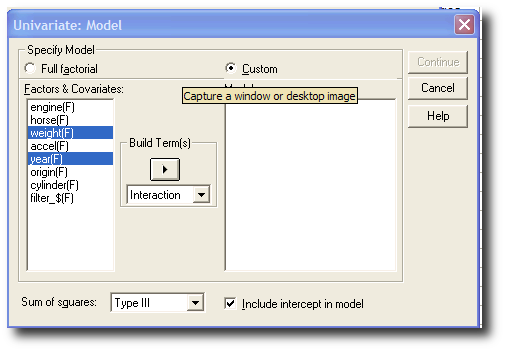
\includegraphics[width=.65\textwidth]{spss-11-model-selection}
 \caption{A dialog box from SPSS version 11 for specifying terms
    for a linear model. The graphic shows a dialog that allows
    the user to specify individual terms in the model  using
    several types of widgets for selection of values, such as a radio
    group, a checkbox, combo boxes, and list boxes. }
  \label{fig:GUI:spss-11-term-selection}
\end{figure}

%% Metaphors, user base
For many \R\/ object types there are natural choices of widget. For
example, values from a sequence map naturally to a slider or spin
button; a data frame maps naturally to a table widget; or a list with
similar structure can map naturally to a tree widget. However, certain
\R\/ types have less common metaphors. For instance, a formula object
can be fairly complex. Figure~\ref{fig:GUI:spss-11-term-selection}
shows an SPSS dialog to build terms in a model. \R\/ power users may
be much faster specifying the formula through a text entry box, but
beginning \R\/ users coming to grips with the command line and the
concept of a formula may benefit from the assistance of a well
designed GUI. One might desire an interface that balances the needs of
both types of user, or the SPSS interface may be appropriate. Knowing
the potential user base is important.







\section{Controls}
\label{sec:GUI:basic-components}
This section provides an overview of many common controls, i.e.,
widgets that represent the actions to be performed on a document. Each
displays some information, and most accept user input.

\subsection{Selection}
\label{sec:GUI:basic-selection}

A common task for a GUI is the selection of a value. In the context of
\R\/, there are many different types of values the user may need to
select. For example, selecting a data frame from a list of data
frames, selecting a variable in a data frame, selecting certain cases
in a data frame, selecting a logical value for a function argument,
selecting a numeric value for a confidence level or selecting a string
to specify an alternative hypothesis. Clearly there can be no
one-size-fits-all widget to handle the selection of a value. We
describe some standard selection widgets next. 


% XXX REDO FIGURE
% \begin{figure}
%   \centering
%   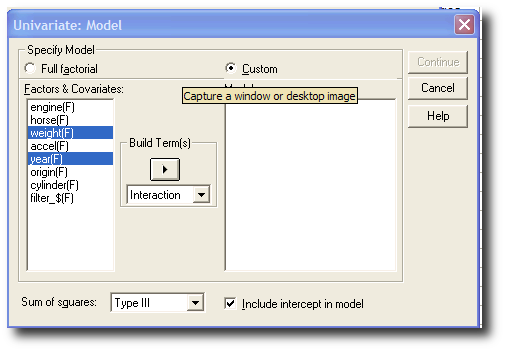
\includegraphics[width=.45\textwidth]{spss-11-model-selection}
%   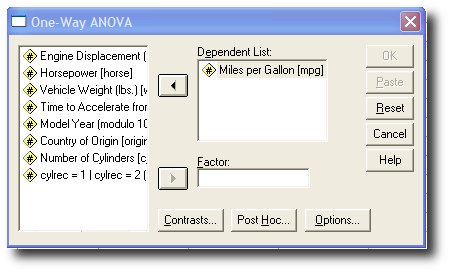
\includegraphics[width=.45\textwidth]{spss-11-one-way-anova}
%   \caption{Two dialog boxes from SPSS version 11 for specifying terms
%     for a linear model. The left graphic shows a dialog that allows
%     the user to specify individual terms in the model. This uses
%     several types of widgets for selection of values, such as a radio
%     group, a checkbox, combo boxes, and list boxes. The right graphic
%     shows a dialog that allows the user to specify response variables
%     and a grouping variable for a one-way ANOVA.}
%   \label{fig:GUI:spss-11-model-selection}
% \end{figure}

\subsubsection{Checkboxes}
\label{sec:GUI:checkboxes}

A \dfn{checkbox} allows the user to select a logical value for a
variable. Checkboxes have labels to indicate which variable is being
selected. Combining multiple checkboxes into a group
allows for the selection of one or more values at a time.  

\subsubsection{Radio Button Groups}
\label{sec:GUI:radio=button-groups}

A \dfn{radio button group} allows a user to select exactly one value
from a vector of possible values. The analogy dates back to old car
radios where there were a handful of buttons to press to select a
preset channel. When a new button was pushed in, the old button popped
up. This safety feature allowed drivers to keep their eyes on the
road.  Radio button groups are useful, provided there are not too many
values to choose from, as all the values are shown. These values can
be arranged in a row, a column or both rows and columns to better use
screen space.

%% tcltk examples
\begin{figure}
  \centering
  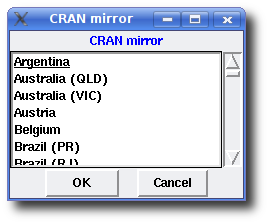
\includegraphics[width=.35\textwidth]{ex-listbox}
  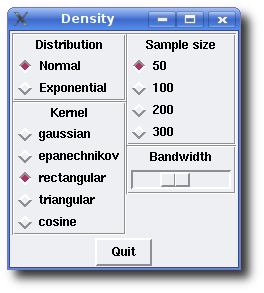
\includegraphics[width=.35\textwidth]{tcltk-tkdensity}
  \caption{
    Two applications of the \pkg{tcltk} package. 
    %%
    The left graphic is
    produced by \command{chooseCRANmirror} and uses a list box to
    allow selection from a long list of possibiulities.
    %% 
    The right graphic is the \code{tkdensity} demo from the
    package. It uses radio buttons and a slider to select the
    parameter values for a density plot.
  }
  \label{fig:GUI:ex-tcltk}
\end{figure}

\subsubsection{Sliders and spinbuttons}
\label{sec:GUI:sliders}

A \dfn{slider} is a widget that selects a value from a
sequence of possible values (typically) through the manipulation of a
knob that can visually range over the possible values. Some toolkits
(e.g. Java/Swing) only allow for the sequence to have integer values. The
slider is a good choice for offering the user a selection of parameter
values. The \code{tkdensity} demo of the \pkg{tcltk} package
(Figure~\ref{fig:GUI:ex-tcltk}) uses a slider to dynamically adjust the
bandwith of a density estimate.


A \dfn{spin button} also allows the user to specify a value from a
possible sequence of values. Typically, this widget is is drawn with a
text box displaying the current value and two arrows to increment or
decrement the selection. The text box can usually be edited. Some
toolkits generalize beyond a numeric sequence. For example, the
letters of the alphabet could be a sequence. A spin button has the
advantage of using less screen space, but is less usable if the
sequence is long, although often the user can enter in the choice
using the keyboard. A spin button is used in the KDE print dialog of
Figure~\ref{fig:GUI:print-dialogs} to adjust the number of copies.


\subsubsection{Combo boxes}
\label{sec:GUI:combo-boxes}

A \dfn{combo box} is a widget that allows the selection of one of
several fixed values, while displaying just the currently selected
one. Comboboxes may also offer the user the ability to specify a
value, in which case they are combined with a text entry area.  From a
screen-space perspective, they can efficiently allow the selection of
a value from many values, although a choice from too many values can
be annoying to the user, such as when a web form requests the
selection of a country from hundreds of choices.

\subsubsection{List boxes}

A \dfn{list box} is a widget that displays in a column the list of
possible choices. A scrollbar is used when the list is too long to
show in the allocated space. Some toolkits have list boxes that allow
the values to spread out over several columns. Selection typically
occurs with a right mouse click or through the keyboad, whereas a
double-click will typically be programmed to initiate some
action. Unlike comboboxes, list boxes can be used for multiple
selection. This is typically done by holding down either the
\kbd{shift} or \kbd{ctrl} keys. Figure~\ref{fig:GUI:ex-tcltk} shows a
list box created by \R\/ that is called from the function
\command{chooseCRANmirror}.

%List boxes are a good alternative to drop lists when the number of
%selections gets bigger than 30. Additionally, 

% ML: what is the rationale for > 30 selections? Drop lists are
% essentially like a list box in that regard.
% JV: I guess personal preference. I took it out.

% Some toolkits allow widgets to be placed next to the entries, such as
% checkboxes or icons. The right-most graphic in
% Figure~\ref{fig:GUI:spss-11-model-selection} shows how SPSS places an icon
% indicating the type of variable next to the variable name in a list
% box, to aid in selection of the proper type of variable.



\subsection{Displaying data}
\label{sec:GUI:tabular-display}

Table and tree widgets support the display and manipulation of tabular
and hierarchical data, respectively. More arbitrary data
visualization, such as statistical plots, can be drawn within a GUI
window, but such is beyond the scope of this section.

%% JV: Need to include filtering example here

\subsubsection{Tabular display}

A \dfn{table widget} shows tabular data, such as a data frame, where
each column has a specific data type and cell rendering strategy.
Table widgets handle the display, sorting and selection of records from a
dataset, and may support editing.  Figure~\ref{fig:GUI:spotfire} shows
a table widget being used in a Spotfire web player demonstration to
display the cases that a user selects through the filtering controls.


\begin{figure}
  \centering
  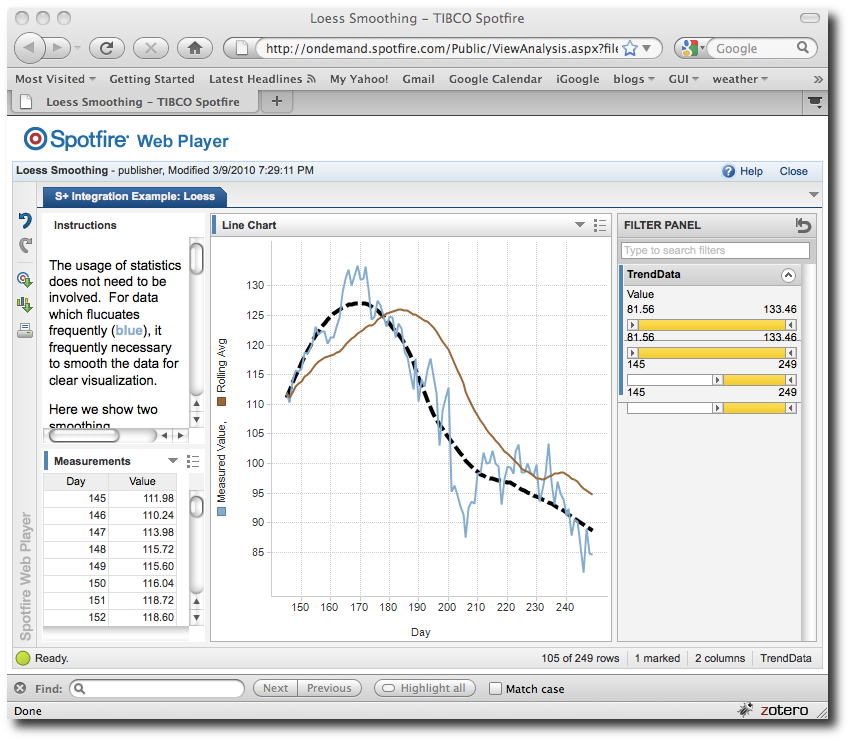
\includegraphics[width=0.8\textwidth]{fig-spotfire}
  \caption{A screen shot from Tibco's Spotfire web player illustrating a table widget (lower left) being used to display the selected cases that are summarized in the graphic. The right bar provides a means to filter the cases under consideration.}
  \label{fig:GUI:spotfire}
\end{figure}


% \begin{figure}
%   \centering
% %%  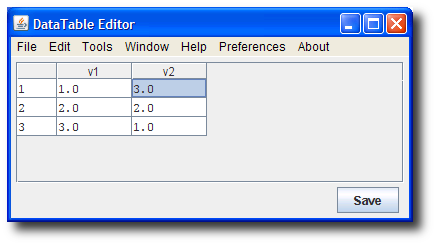
\includegraphics[width=.4\textwidth]{JGR-data-editor}
%   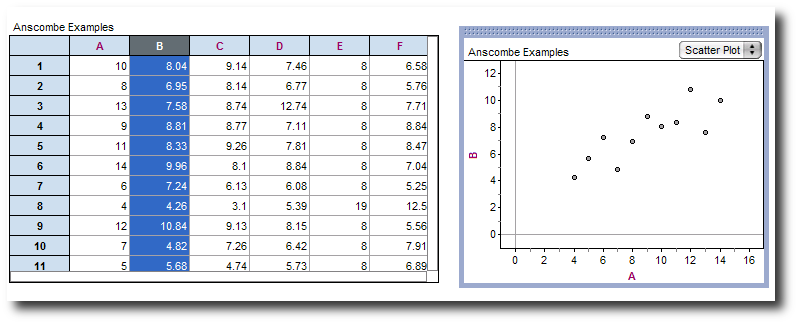
\includegraphics[width=.55\textwidth]{fathom-2-1-xyplot}
%   \caption{
%     Two windows showing the use of table widgets.
%     %%
    
% %     The left graphic shows the data editor from \pkg{JGR} using the
% %     table widget in Java.  
%     %%
%     The right graphic shows a data table and a graph in Fathom 2.1
%     with two views of the same data. One view uses a table widget, the
%     other a graph. Changes to one or the other views cause an update
%     to the underlying model. This model then will notify its various
%     displays to update. This arrangement allows for dynamic linking of
%     the table and the graph.}
%   \label{fig:GUI:table-widgets}
% \end{figure}

\subsubsection{Tree widgets}
\label{sec:GUI:tree-widgets}

So far, we have seen how list boxes display homogeneous vectors of
data, and how table widgets display tabular data, like that in a data
frame. Other widgets support the display of more complex data
structures. If the data has a heirarchical structure, then a \dfn{tree
  widget} may be appropriate for its display. Examples of heirarchical
data in \R, are directory structures, the components of a list, or
class hierarchies. The object browser in \pkg{JGR} uses a tree
widget to show the components of the objects in a users session (the
left graphic of Figure~\ref{fig:GUI:R-guis-exs-JGR-Rcmdr}). The root
node of the tree is the ``data'' folder, and each data object in the
global workspace is treated as an offspring of this root node. For the
data frame \code{iraq}, its variables are considered as offspring of
the data frame. In this case these variables have no further
offspring, as indicated by the ``page'' icon.


\subsection{Inititiating an action}

After the user has specified the parameters of an action, typically
through the selection widgets presented above, it comes time to
execute the action. Widgets that execute actions include the familiar
buttons, menubars and toolbars.


\subsubsection{Buttons}
\label{sec:GUI:buttons}

A \dfn{button} is typically used to give the user a place to click the
mouse in order to initiate some immediate action. The ``Properties''
button, when clicked, opens a dialog for setting printer
properties. The button with the wizard icon also opens a dialog.  As
buttons typically lead to an action, they often are labeled with a
verb.~\citep{APPLE:HIG} In Figure~\ref{fig:GUI:spss-11-term-selection}
we see how SPSS uses buttons in its dialogs: buttons which are not
valid in the current state are disabled; buttons which are designed to open
subsequent dialogs have trailing dots; and the standard actions of
resetting the data, canceling the dialog or requesting help are given
their own buttons on the right edge of the dialog box.  

To speed the user through a dialog, a button may be singled out as the
default button, so its action will be called if the user presses the
\kbd{return} key. As well, buttons may be given accelerator key
bindings, so as their actions are accesible by typing the proper key
combination. The KDE print dialog in
Figure~\ref{fig:GUI:print-dialogs} has these bindings indicated
through the underlined letter on the button label's.

%% ML: besides the accelerator comment, the below might be too much detail
%% JV: I'll leave it for the toolkit chapters if appropriate.
%% adjustments
% The look of the button can usually be manipulated.  A button is given
% a relief through its border, shading, and perhaps a color gradient
% along its face. Some toolkits allow these to be optionally drawn,
% thereby making a button look more like a label, as described below.
% The button text may have some markup or an indication of a accelerator
% keyboard binding, such as the \text{\underline{C}ontrasts...} button
% in the dialog shown in the right graphic of
% Figure~\ref{fig:GUI:spss-11-model-selection}.

\subsubsection{Icons}
\label{sec:GUI:icons}

In the WIMP paradigm, an \dfn{icon} is a pictorial representation of a
resource, such as a document or program, or, more generally, a
concept, such as a type of file. An application GUI typically adopts
the more general definition, where an icon is used to augment or
replace a text label on a button, a toolbar, in a list box, etc. When
icons are used on toolbars and buttons, they are associated with
actions, so the icons should have some visual implication of an
action.  Well chosen icons make a big visual difference in a GUI.

% ML: too much detail?
% JV: agreed
% Except for the default installation of \pkg{tcltk}, images and icons
% may be specified in a variety of different formats.  Icons can come in
% several different sizes from 16 by 16 pixels to 128 by 128. For
% toolbars and menubars, the toolkit takes care of selecting the
% appropriate icon.


\subsubsection{Menubars}
\label{sec:GUI:menubars}

Xerox Parc's revolutionary idea of a \acronym{WIMP} GUI added windows,
icons, menubars, and pointing devices to the desktop computing
environment. The central role of menu bars has not diminished. For a
GUI, the \dfn{menubar} gives access to the full range of functionality
available. Each common action should have a corresponding menu
item. Menubars are traditionally associated with a top-level
window. This is enforced by the toolkit in \wxWidgets\/ and \Java\/
but not \tcltk\/ and \GTK.  In Mac OS X, the menubar appears on the
top line of the display, but otherwise they typically appear at the
top of the main window. In most modern applications, standard
document-based design is used to organize a GUI and its actions, with
a main window showing the document and its menu bar calling actions on
the document, some of which may need to open subsequent application
windows or dialogs for gathering additional user input.  In this
model, only the main window has a menu bar, not the application
windows or dialogs. In a statistics application, the ``document'' may
be viewed as the active data frame, a report, or a graphic.

The styles used for menubars are fairly standardized, as this allows
new users to quickly orient themselves with a GUI. The visible menu
names are often in the order \code{File}, \code{Edit}, \code{View},
\code{Tools}, then application specific menus, and finally a
\code{Help} menu. Each visible menu item when clicked opens a menu of
possible actions. The text for these actions traditionally use a
\code{...}  to indicate that a subsequent dialog will open so that
more information can be gathered to complete the action, as opposed to
some immediate action being taken. The text may also indicate a
key-board accelerator, such as \code{Find \underline{N}ext F3}
indicating that both ``N'' as a keyboard accelerator and F3 as a
shortcut will initiate this same action.

Not all actions will be applicable at any given time. It is
recommended that rather than deleting these menu items, they be
disabled, or greyed out, instead. %%~\ref{KDE:HIG}

Menus can get very long. To help the user navigate, menu items are usually
grouped together, first by being under the appropriate menu title,
then with either horizontal separators to define subsequent groupings,
or hierarchical submenus. The latter are indicated with an
arrow. Several different levels are possible, but navigating through
too many can be tedious.

The use of menus has evolved to also allow the user to set properties
or attributes of current state of the GUI. There may be checkboxes
drawn next to the menu item or some icon indicating the current state.

Another use of menus is to bind contextual menus (popup menus) to
certain mouse clicks on GUI elements. Typically right mouse clicks
will pop up a menu that lists often-used commands that are appropriate
for that widget and the current state of the GUI. In Mac OS X
one-button users, these menus are bound to a \kbd{control}-click.

\subsubsection{Toolbars}
\label{sec:GUI:toolbars}

Toolbars are used to give immediate access to the frequently used actions
defined in the menubar. Toolbars typically have icons representing the
action and perhaps accompanying text. They traditionally appear on the
top of a window, but sometimes are used along the edges. 


%%%%%%%%%%%%%%%%%%%%%%%%%%%%%%%%%%%%%%%%%%%%%%%%%% 
\subsection{Displaying and editing text}
\label{sec:GUI:text-widgets}

As much as possible, WIMP GUIs are designed around using the pointing
device to select values for user input. Perhaps this is because it is
difficult to both type and move the mouse at the same time. For
statistical GUIs, especially for \R\/ with its powerful command line,
the flexibity afforded by arbitrary text entry is essential for any
moderately complex GUI. There is a distinction made between widgets
for handling just single lines versus multiple lines of text.

\subsubsection{Single line text}
\label{sec:GUI:single-line-text}

A text entry widget for editing a single line of text is used in the
KDE print dialog (Figure~\ref{fig:GUI:print-dialogs}) to specify
the page range. As range's can be complex to specify, the command line
has an advantage. A disadvantage of using this type of widget is the need to
validate the user's input, as the input must conform to some specfication.

\subsubsection{Text edit boxes}
\label{sec:GUI:textboxes}

Multi-line text entry areas are used in many GUIs. The right graphic
of Figure~\ref{fig:GUI:R-guis-exs-JGR-Rcmdr} shows a text entry area
used by \pkg{Rcmdr} to enter \R\/ commands, to show the output of the
commands and to provide a message area (in lieu of a status bar). The
``Output Window'' demonstrates the utility of formatting
attributes. In this case, attributes are used to specify the color of
the commands, so that the input can be distinguished from the output.

\begin{figure}
  \centering
  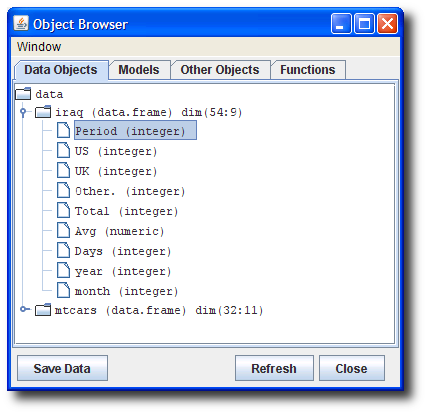
\includegraphics[width=.35\textwidth]{JGR-object-browser}
  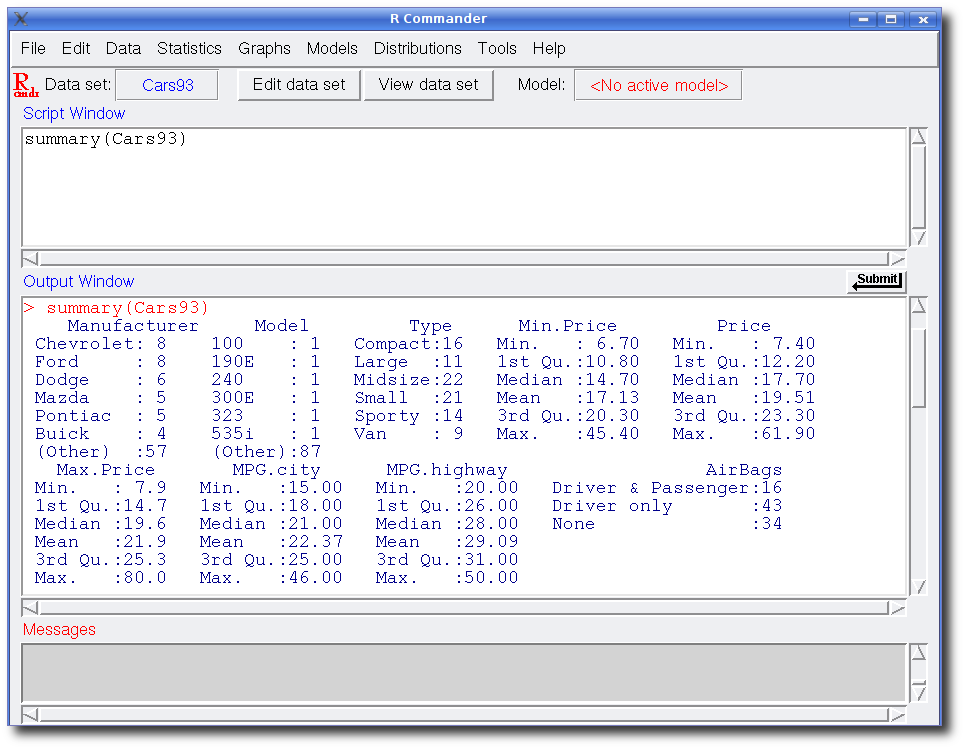
\includegraphics[width=.5\textwidth]{Rcmdr-main-window}
  \caption{
    Some windows from \R\/ GUIs.
    %% 
    The left graphic shows the object browser in the \pkg{JGR} GUI
    using a tree widget 
    to display the possibly heirarchical nature of \R\/ objects.
    %%
    The right graphic shows the main Rcmdr (1.3-11) window
    illustrating the use of multi-line text entry areas for a command
    area, an output area and a message area.}
  \label{fig:GUI:R-guis-exs-JGR-Rcmdr}
\end{figure}


\XXX{Not needed here?}
% %% A table showing the values and constructors
% %% Make changes to gnumeric spreadsheet, export
% {\small
% \newcommand{\PARASIZE}{1.25in}
% \newcommand{\LARGEPARASIZE}{1.45in}
% \begin{landscape}
%   \begin{table}[tbp]
%     \centering
%     \begin{minipage}{1.0\textwidth}
%       \begin{tabular}{lp{\PARASIZE}@{\quad}p{\LARGEPARASIZE}@{\quad}p{\PARASIZE}@{\quad}p{\PARASIZE}@{\quad}p{\PARASIZE}@{\quad}c}
%         %%
%         Widget & \code{gWidgets} & \code{RGtk2} & \code{RwxWidgets} &
%         \code{tcltk}~\footnote{Some constructors require add-on
%           libraries, as indicated by parentheses.} & \code{rJava} &\\
%         \hline
%         \SweaveInput{widgets-constructors}
%       \end{tabular}
%     \end{minipage}
%     \caption{A table listing several common widgets with a constructor for
%       different toolkits discussed in the text.}
% \label{tab:GUI:widgets-constructors}
%   \end{table}
% \end{landscape}
% }

%%%%%%%%%%%%%%%%%%%%%%%%%%%%%%%%%%%%%%%%%%%%%%%%%% 
\subsection{Display of information}
\label{sec:GUI:info-display}

Some widgets are typically used to just display information and often
do not respond to mouse clicks. These are called static controls in
\wxWidgets.

\subsubsection{Labels}
\label{sec:GUI:labels}
%% Static Text
A label is a widget for placing text into a GUI that is typically not
intended for editing, or even selecting with a mouse. This widget is
used to label other controls, so the user understands what will happen
when that control is changed.

%% markup
A Label's text can be marked up in some
toolkits. Figure~\ref{fig:GUI:Rcmdr-main-window} shows labels marked
in red and blue in \pkg{tcltk}.

\subsubsection{Statusbars}
\label{sec:GUI:statusbars}

A typical top-level window will have a menubar and toolbar for access
to the possible actions, an area to display the document being worked
on, and at the bottom of the window a statusbar for giving the user
immediated feedback on the actions that have been
initiated. 

\subsubsection{Progress bars}

A progress bar is used to indicate the percentage of a particular task
that has been completed. They are often used during software installation. 


\subsubsection{Tooltips}
\label{sec:GUI:basic-tooltips}

A tooltip is a small window that pops up when a user hovers their
mouse over a tooltip-enabled widget. These are useful for providing
extra information about a particular piece of content displayed by a
widget. A common use-case is to guide new users of a GUI. Many
toolkits support the display of interactive hypertext in a tooltip,
which allows the user to request additional details.

%% combined with modal dialogs
% \subsection{Choosers}
% \label{sec:GUI:choosers}

% Certain standard widgets are used to select values from a range
% defined by the system the user is on.


% \subsubsection{Color choosers}
% \label{sec:GUI:color-pickers}

% A color picker allows the selection of a color. 

% \subsubsection{Font choosers}
% \label{sec:GUI:font-choosers}

% A font chooser allows the selection of a font. 


\subsection{Modal dialog boxes}
\label{sec:GUI:modal-dialogs}

A \dfnref{modal dialog box} is a dialog box that keeps the focus until
the user takes an action to dismiss the box. They are used to notify
the user of some action, perhaps asking for confirmation in case the
action is destructive, such as overwriting of a file name. Modal
dialog boxes can be disruptive to the flow of interaction, so they
should be used sparingly. As the flow essentially stops until the
window is dismissed, functions that call modal dialogs can return a
value when an event occurs, rather than have a handler respond to the
dismiss event. The \command{file.choose} function, mentioned below, is
a good example. When used during an interactive \R\/ session, the user
is unable to interact with the command line until a file has been
specified and the dialog dismissed.


\subsubsection{File choosers}
\label{sec:GUI:file-choosers}

A file chooser allows for the selection of existing files, existing
directories, or specifying the name of a new file. They are familiar to
any user of a GUI. A typical \R\/ installation has the functions
\command{file.choose} and \command{tkchooseDirectory} (in the
\pkg{tcltk} package) to select files and directories.


Other common choosers are color choosers and font choosers.

\subsubsection{Message dialogs}
\label{sec:GUI:message-dialogs}

A \dfnref{message dialog} is a high-level dialog widget for
communicating a message to the user. Generally, it has a standard
form. There is a small rectangular box that appears in the middle of
the screen with an icon on the left and a message on the right. At the
bottom is a button to dismiss the dialog, often labeled ``OK.'' The
\dfnref{confirmation dialog} variant would add a ``Cancel'' button
which invalidates the proposed action.



\section{Containers}
\label{sec:GUI:basic-components-containers}
%% Containers

%% ML: Layout management is orthogonal to the type of container. This
%% is made obvious in the design of Swing and Qt: there is a separate
%% class hierarchy for layout managers, which are assigned to
%% container widgets. The container could be invisible or provide an
%% interface around its children, as with a frame, notebook or top-level
%% window. Thus, in Qt, a frame container could lay out its children
%% as a box, a grid, etc. I suggest discussing container types first,
%% and then discuss layout management policies, explaining that some
%% toolkits have widgets specific to a particular policy (and so
%% require a lot of nesting), while in others any container type is
%% capable of any type of layout.


%% JV: good point. 
% Widgets are arranged in a window to produce a GUI. Container widgets
% manage the layout. The simplest containers are like boxes
% that get packed in left to right or top to bottom. These boxes may be
% decorated with a frame or label, or may have some means of being
% hidden or displayed by the user. The nesting of box containers can
% provide a great deal of flexibility, but usually not
% enough. An example of a more flexible layout strategy is to position
% widgets on a grid.

%% Widget Heirarchy

Widgets in a GUI are organized in a \dfn{widget heirarchy}, where some
widgets are parents and some children (which may in turn be
parents). The top-level window may play a special role here, as a
parent but not a child. This organization offers the toolkit writers
the chance to treat each object as a standalone component. For
example, when a GUI is resized the typical algorithm is for the parent
to be resized, then to send a signal to the children to resize
themselves. Another example is when a window is closed, prior to
closing the window will signal its children that they will be
destroyed, and they should in turn signal their children, if any.  A
means to traverse the widget heirarchy is provided by each toolkit.
In \pkg{tcltk} this heirarchical relationship is explicit, as a widget
constructor -- except for top-level windows -- requires a parent
widget when be constructed. In the other toolkits, it may be implicit.

In the widget heirarchy, the parents play a different role as those
widgets that are just children. The parents play the role of
\dfn{containers}. Sometimes the word \dfn{widget} is reserved for GUI
components which are not-containers. Having containers makes it
possible to organize GUIs into indivividual components -- again, a desirable
design feature.

The children of the GUI must be organized in some manner. In \GTK
(\pkg{gWidgets}), this is done through the choice of container with
parameters being set to adjust the placement within the container when
the child is added. In \Qt\/ and \tcltk\/ there is an added
abstraction of a layout. A layout decouples the heirarchy from the
layout and offers much more flexibility. In \Qt\/ this allows for a
richer set of default layout options, and the ability to create ones
specialized layouts.



\subsection{Top level windows}
\label{sec:GUI:top-level-windows}

The top-level window of a GUI is typically decorated with a title and
buttons to iconify, maximize, or close. Besides the text of the title,
the decorations are generally the domain of the window manager, often
part of the operating system. The application controls the contents of
the window. Generally, a top-level window will consist of a menu bar,
a tool bar and a status bar. In between these is the area referred to
as the \dfnref{client area} or \dfnref{content pane} where other
containers or widgets are placed.

%% client area -- wxWidgets book
%% content pane -- java tutorial

%% FRAME vs. WINDOW

%% closing property

The title is a property of the window and may be specified at the time
of construction or afterwards. 

On a desktop, only one window may have the focus at a time. It may or
may not be desired that a new window receive the focus so some means
to specify the focus at construction or later is provided by the
toolkit.

The initial placement of the window also may be specified at the time
of construction. The top-level window of a GUI may generally be placed
whereever it is convenient for the user, but sub-windows are often
drawn on top of their parent window, as are modal dialog boxes. 


%% RGtk2 -- DefaultSize
%% rJava -- Preferred Size
%% tcltk -- min size
%% RwxWidgets -- DefaultSize

%% ML: I don't think that the ability to set a default or minimum size
%% depends on the toolkit. It's all determined by the windowing system
%% and what the associated window managers are required to support. I
%% would say that on all major platforms, one can set both a default
%% and a minimum size, as well as toggle resizability, with any
%% reasonable toolkit. Certainly this is true of GTK+ and Qt. The
%% top-level window geometry is the result of negotiation between the
%% window manager and application.

The window manager usually decorates a top-level window with a close
button. It may be necessary or desirable to specify some action to
take place when this button is clicked. For instance, a user might be
prompted if they wish to save changes to their work when the close
button is pressed.

it may take some time to initially layout a top-level window. Rather
than have the window drawn and then have a blank window while this
time passes, it is preferable to not make the window visible until the
window is ready to draw. 


We now describe some of the main containers.

% Table~\ref{tab:GUI:containers-constructors} lists them
% together and provides the constructor name for the different toolkits
% discussed in this book.

\subsection{Box containers}
\label{sec:GUI:Box-containers}

A box container places its children in it from left to right or from
top to bottom.  If each child is viewed as a box, then this container
holds them by packing them next to each other. The upper left figure in
Figure~\ref{fig:GUI:box-possibilities} illustrates this. 

When the boxes have different sizes, then some means to align them
must be decided on. Several possibilities exists. The alignment could
be around some center, aligned at a baseline, the top line, or each
child can specify where to anchor itself within the allotted space
(the upper right graphic in Figure~\ref{fig:GUI:box-possibilities}).

If the space allocated for a box is larger than the space requested by
a child component then a decision as to how that component gets placed
needs to be made. If the component is not enlarged, then there are
nine reasonable places -- the center and the 8 compass directions N,
NW, W, \dots. Otherwise, it may be desirable for the component to
expand horizontally, vertically or both (the lower left graphic in
Figure~\ref{fig:GUI:box-possibilities}). Additionally, it is desirable
to be able to place a fixed amount of space between child components
or a spring between components. A spring forces all subsequent to
children to the far right or bottom of the container (the lower right
graphic in Figure~\ref{fig:GUI:box-possibilities}).


When a top-level window is resized, these space allocations must be
made. To help, the different toolkits allows the components to have a
size specifed. Some combination of a minimum size, a preferred size, a
default size, a specific size, or a maximum size are
allowed. Specifying fixed sizes for components is generally frowned
upon, as they don't scale well when a user resizes a window and they
don't work well when different languages are used on the controls when
an application is localized.


\begin{figure}
  \centering
  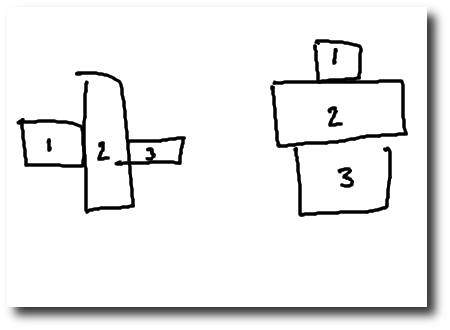
\includegraphics[width=.35\textwidth]{box-horizontal}
  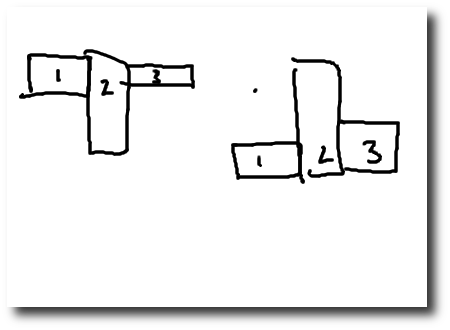
\includegraphics[width=.35\textwidth]{box-alignment}\\
  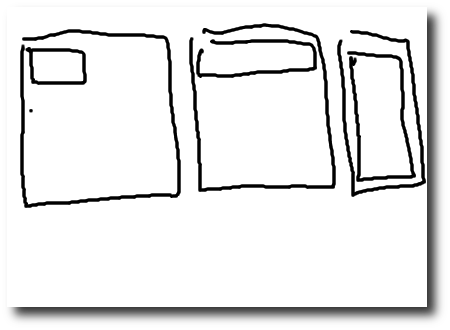
\includegraphics[width=.35\textwidth]{box-expand}
  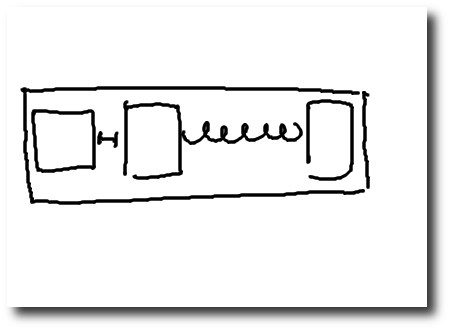
\includegraphics[width=.35\textwidth]{box-glue-spring}
  \caption{
    XXX REPLACE WITH REAL GRAPHICS XXX.
    %%
    Different possibilities for packing child components within
    a box. 
    %%
    The upper left shows horizontal and vertical layout.
    %% 
    The upper right shows some possible alignements.
    %%
    The lower left shows that a child could possibly be anchored in
    one of 9 positions. As well, it could ``expand'' to fill the space
    either horizontally (as shown) or  vertically, or both.
    %%
    The lower right shows both a fixed amount of space between the
    children and an expanding spring between the child components.
}
  \label{fig:GUI:box-possibilities}
\end{figure}

\subsubsection{Frames}
\label{sec:GUI:frames}

A box container may have a border drawn around it to visually separate
its contents from others. This border may also have a title. In
\GTK\/ these are called frames, but this word is reserved in \tcltk\/ and
\Java.

\subsubsection{Expanding boxes}
\label{sec:GUI:expanding-boxes}

In order to save screen space, a means to hide a boxes contents can be
used. This hiding/showing is initiated by a mouse click on a
disclosure button or trigger icon.

\subsubsection{Paned boxes}
\label{sec:GUI:paned-boxes}

If automatic space allocation between two child components is not
desired, but rather a means for the user to allocate the space is,
then a \dfnref{paned container} may be used. These offer one or more
horizontal or verticales sash that can be clicked and dragged to
apportion space between the child omponents.

   
\subsection{Grid layout}
\label{sec:GUI:grid-layout}

By nesting box containers, a great deal of flexibility in layout can
be achieved. However, there is still a need for the alignment of child
components in a tabular manner. The most flexible alignments allow for
different sizes for each column and each row, and additionally, the
ability for the child components to span multiple columns or
rows. Within each cell (or cells) the placement of a child component
mirrors that of the lower left graphic of
Figure~\ref{fig:GUI:box-possibilities}. Some specification where to
anchor the component when there are nine possible positions plus
expanding options must made.

\subsection{Tabbed Notebooks}
\label{sec:GUI:notebooks}

A notebook is a common container to hold one or more pages (or
children). The different pages are shown by the user through the
clicking of a corresponding tab. The metaphor being a tabbed
notebook. Modern web browsers take advantage of this container to
allow several web pages to be open at once.




\subsection{Example}

The KDE pring dialog of Figure~\ref{fig:GUI:print-dialogs} shows
most of the containers previously described. 

The top-level window has the generic title ``Print -- KPDF.'' This
window appears to have four child components: a frame labeled
\code{Printer}, a notebook with open tab \code{C\underline{o}pies}, a
grid layout for specifying the print system, and a box for holding
five buttons at the bottom. 

The lower left \code{\underline{O}ptions} button has \verb+<<+ to
indicate that clicking this will close an exanding box, in this case a
box that contains the lower three components above. So in fact, there
are two visible child components of the top-level window.

The framed box holds a grid layout with five columns and 6 rows. The
sizes allocated to each column are visible in the first row. It is
quickly seen that each column has a different size. The last row has a
text entry area that spans the second and third columns. The first
column has only labels. These are anchored to the left side of the
allowed space. The Apple human interface guide
\citep{APPLE:HIG} suggests using colons for text that provides
context for controls, and the KDE designers do to. 

The displayed page of the notebook shows two child components, both
framed boxes. A pleasant amount of space between the frames and their
child components has been chosen. The \code{Page Selection} frame has
components including radio buttons, a text area, a horizontal
separator, and a combo box.

The print system information is displayed in a grid layout that has
been right aligned within its parent container -- the expanded group,
but its children are center-balanced with the label ``Print system
currently used'' is right aligned and ``Server...'' is left aligned
within their cells.

The button box shows five buttons as child components. At first glance
the sizing appears to show that each button is drawn to fully show its label
with some fixed space placed between the buttons. If the dialog is
expanded, it is seen that there is a spring between the 3rd and 4th
buttons, so that the first 3 are aligned with the left side of the
window and the last two the right side.

% The Apple guidlines\citep[Ch. 15]{APPLE:HIG} suggest using ``center
% equalization'' for arranging widgets within a window. This means that
% the visual weight is balanced between the right and left side of the
% content area. This is not the case with the KDE print dialog.



% %% A table showing the values and constructors
% %% Make changes to gnumeric spreadsheet, export
% {\small
% \newcommand{\PARASIZE}{1.25in}
% \begin{landscape}
%   \begin{table}
%     \centering
%     \caption{A table listing several containers with a constructor for the
%       different toolkits discussed in the text.}
%     \begin{tabular}{lp{\PARASIZE}@{\quad}p{\PARASIZE}@{\quad}p{\PARASIZE}@{\quad}p{\PARASIZE}@{\quad}p{\PARASIZE}@{\quad}c}
% Widget & \code{gWidgets} & \code{RGtk2} & \code{RwxWidgets} &
% \code{tcltk} & \code{rJava} &\\
% \hline
% \SweaveInput{containers-constructors}
%     \end{tabular}
% \label{tab:GUI:containers-constructors}
%   \end{table}
% \end{landscape}
% }


\section{End of chapter notes}
\label{sec:GUI:end-of-chapter}
\XXX{ fill this in }

More documentation on GUIs is available in book format or online. 

For \GTK\/ there is the gtk tutorial (pygtk); GTK API; DTL's notes; example
code in the \pkg{RGtk2} package; php-gtk cookbook

For \wxWidgets the book; DTL omegahat pages; wxWidgets API;

For \tcltk\/ ActiveStates API; wettenhall examples (sciviews);
Dalgaard's papers; R mailing list; book

For \Java\/ Sun's website tutorials; API; rJava package page; 

Event loops




%%%%%%%%%%%%%%%%%%%%%%%%%%%%%%%%%%%%%%%%%%%%%%%%%%

